\documentclass[preprint,12pt]{elsarticle}

\usepackage{amssymb}
\usepackage{amsmath}
\usepackage{amsthm}
\usepackage[utf8]{inputenc}
\usepackage{lmodern}
\usepackage{graphicx}
\usepackage{xurl}
\usepackage[hidelinks]{hyperref}

\journal{European Journal of Combinatorics}
\makeatletter
\def\ps@pprintTitle{\let\@oddhead\@empty\let\@evenhead\@empty
  \def\@oddfoot{\footnotesize\itshape Author manuscript\hfill 25 October 2026}
  \let\@evenfoot\@oddfoot}
\makeatother


\newcommand{\releaseURL}{https://github.com/creelie/automatic-memory/releases/tag/v2.2.0}

\newtheorem{theorem}{Theorem}[section]
\newtheorem{proposition}[theorem]{Proposition}
\newtheorem{lemma}[theorem]{Lemma}
\newtheorem{corollary}[theorem]{Corollary}
\newtheorem{conjecture}[theorem]{Conjecture}
\theoremstyle{definition}
\newtheorem{definition}[theorem]{Definition}
\newtheorem{remark}[theorem]{Remark}
\newtheorem{example}[theorem]{Example}

\newcommand{\Q}{\mathbb{Q}}
\newcommand{\Z}{\mathbb{Z}}
\newcommand{\N}{\mathbb{N}}
\newcommand{\g}{\mathfrak{g}}
\newcommand{\slt}{\mathfrak{sl}(2)}
\newcommand{\Ue}{U(\g)}
\newcommand{\tr}{\operatorname{tr}}
\newcommand{\cro}{\operatorname{cr}}
\newcommand{\cyc}{\operatorname{cyc}}
\newcommand{\des}{\operatorname{des}}
\newcommand{\dd}{\partial}
\newcommand{\binomset}[2]{\tbinom{#1}{#2}}

\begin{document}

\begin{frontmatter}

\title{The \texorpdfstring{$\mathfrak{sl}(2)$}{sl(2)} weight system at \texorpdfstring{$c=-3/32$}{c=-3/32} extends to a graph 4-invariant}

\author[egspl,ucal]{Deep Bhattacharjee\corref{cor1}\fnref{orcid1}}
\ead{itsdeep@live.com}
\ead{d.bhattacharjee@erl-forschung.de}
\fntext[orcid1]{ORCID: \url{https://orcid.org/0000-0003-0466-750X}}
\cortext[cor1]{Corresponding author.}
\affiliation[egspl]{organization={Formerly, Electro-Gravitational Space Propulsion Laboratory (EGSPL)},
            city={Bhubaneswar},
            postcode={751030},
            state={Odisha},
            country={India}}
\affiliation[ucal]{organization={Formerly, University of Calcutta},
            addressline={Senate House, 87/1 College Street},
            city={Kolkata},
            postcode={700073},
            state={West Bengal},
            country={India}}

\author[ntu]{Ushashi Bhattacharya\fnref{orcid2}}
\ead{rai.bhattacharya.in@gmail.com}
\fntext[orcid2]{ORCID: \url{https://orcid.org/0009-0002-2254-3914}}
\affiliation[ntu]{organization={Formerly, National Taiwan University},
            city={Taipei},
            postcode={106319},
            country={Taiwan}}

\begin{abstract}
We prove unconditionally the conjecture of Fomichev, Karev, Pavutnitskiy and Usanov that the specialization of the $\mathfrak{sl}(2)$ weight system at $c=-3/32$ extends to a $4$-invariant of graphs. The extension is $\xi(G)=(-32)^{-n}S_G(-2)$, where $S_G(N)$ counts with signs the assignments of $2$-element subsets of $\{1,\dots,N\}$ to the $n$ vertices of $G$.
\end{abstract}

\begin{keyword}
weight system \sep intersection graph \sep four-term relation \sep oscillator representation \sep Clifford algebra
\MSC[2020] Primary 05C31 \sep Secondary 57K16 \sep 17B10 \sep 15A66
\end{keyword}

\end{frontmatter}

\section{Introduction}\label{sec:intro}

A weight system is a function on chord diagrams that satisfies the four-term relations; weight systems are the symbols of finite type knot invariants \cite{Kon93,BN95,CDM12}. A metrized Lie algebra gives a weight system with values in the centre of its universal enveloping algebra. For $\slt$ with the Killing form the centre is the polynomial ring $\Q[c]$ in the Casimir element $c$, and the value $w_D\in\Q[c]$ of the weight system on a chord diagram $D$ depends only on the intersection graph $\Gamma(D)$ \cite{ChL07}. Lando's four-term relations for graphs \cite{Lan00} are such that every function $f$ on graphs satisfying them gives a weight system $D\mapsto f(\Gamma(D))$; such $f$ are called $4$-invariants. Lando asked whether $w$ is obtained in this way \cite{ChL07}; see \cite{KL22} for a survey and \cite{Kra21} for graphs with at most $8$ vertices.

Fomichev, Karev, Pavutnitskiy and Usanov \cite{FKPU} answered the question negatively. They found a linear combination of intersection graphs that vanishes modulo the four-term relations of graphs and on which $w$ takes the value $c(c-\frac38)(c-1)(c+\frac{3}{32})$. Hence the specialization of $w$ at $c=c_0$ can extend to a $4$-invariant only if $c_0\in\{0,\frac38,1,-\frac{3}{32}\}$. For $c_0=0,\frac38,1$, the eigenvalues of the Casimir element on the irreducible representations of dimension $1,2,3$, extensions are known \cite{FKPU,FK25,YDJ26}. The value $-\frac{3}{32}$ is the eigenvalue of the Casimir element on the oscillator representation. The authors of \cite{FKPU} constructed an extension for graphs with at most $10$ vertices and stated:

\begin{conjecture}[{\cite[Section~4]{FKPU}}]\label{conj:fkpu}
The specialization of the $\slt$-weight system at $c=-\frac{3}{32}$ extends to a $4$-invariant of graphs $\xi(G)$.
\end{conjecture}

We prove Conjecture~\ref{conj:fkpu} with an explicit formula. All graphs are finite and simple. For $N\in\N$ write $[N]=\{1,\dots,N\}$ and $\binomset{[N]}{2}$ for the set of its $2$-element subsets.

\begin{definition}\label{def:S}
For a graph $G=(V,E)$ and $N\in\N$ put
\[
S_G(N)=\sum_{p\colon V\to\binomset{[N]}{2}}\ \prod_{xy\in E}(-1)^{|p(x)\cap p(y)|},
\]
and for $k\in\N$ let $T_k(G)$ be the same sum restricted to the maps $p\colon V\to\binomset{[k]}{2}$ with $\bigcup_{x\in V}p(x)=[k]$.
\end{definition}

\begin{theorem}\label{thm:main}
Let $G=(V,E)$ be a graph with $n$ vertices.
\begin{enumerate}
\item[(a)] $S_G(N)=\sum_{k=0}^{2n}\binom{N}{k}T_k(G)$ for all $N\in\N$; thus $S_G$ is a polynomial in $N$ of degree at most $2n$.
\item[(b)] The graph invariant
\[
\xi(G)=\frac{S_G(-2)}{(-32)^{n}}=\frac{1}{(-32)^{n}}\sum_{k=0}^{2n}(-1)^k(k+1)\,T_k(G)
\]
satisfies the four-term relations of graphs.
\item[(c)] For every chord diagram $D$, $w_D(-\frac{3}{32})=\xi(\Gamma(D))$.
\end{enumerate}
\end{theorem}

Parts (b) and (c) are Conjecture~\ref{conj:fkpu}. The two expressions for $\xi$ agree by (a), since $\binom{-2}{k}=(-1)^k(k+1)$.

\begin{example}\label{ex:small}
For one vertex, $S_{K_1}(N)=\binom N2$ and $\xi(K_1)=3/(-32)=-\frac{3}{32}$, the value of $w$ on one chord. Since $S_{G\sqcup H}=S_GS_H$, $\xi$ is multiplicative, as $w$ is. For two adjacent vertices, the pairs $(p(x),p(y))$ with $|p(x)\cap p(y)|=2,1,0$ number $\binom N2$, $\binom N2\cdot 2(N-2)$ and $\binom N2\binom{N-2}{2}$, so $S_{K_2}(N)=\binom N2\bigl(1-2(N-2)+\binom{N-2}{2}\bigr)$ and $\xi(K_2)=3\cdot19/1024=\frac{57}{1024}$. This is $c(c-\frac12)$ at $c=-\frac{3}{32}$, the value of $w$ on two crossing chords.
\end{example}

\begin{figure}[ht]
\centering
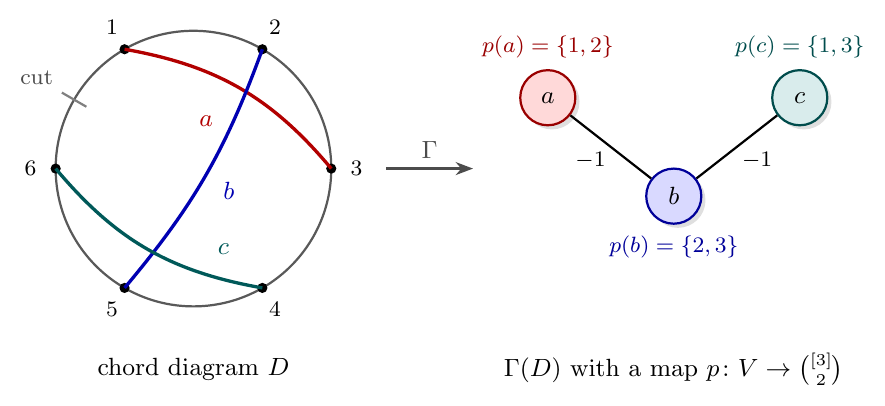
\includegraphics[width=0.92\textwidth]{figures/fig_chords.png}
\caption{A chord diagram with three chords, cut between the points $6$ and $1$, and its intersection graph, a path. The map $p$ sends each vertex to a $2$-element subset of $[3]$; both edges meet in one element, so $p$ contributes $(-1)(-1)=1$ to $S_{\Gamma(D)}(3)$.}\label{fig:chords}
\end{figure}

The proof of (b) is an involution on assignments (Section~\ref{sec:proof}). For (c) we let the element $C_D\in U(\slt)$ of a chord diagram act on the Verma module of highest weight $\mu$; it acts by a polynomial $\lambda_D(\mu)$, and $w_D(-\frac{3}{32})=\lambda_D(-\frac12)$ (Section~\ref{sec:verma}). The oscillator representation on $\Q[z]$ is the sum of the Verma modules of highest weights $-\frac12$ and $-\frac32$, so the image of $C_D$ in the Weyl algebra is the scalar $\lambda_D(-\frac12)$. A supertrace on the Weyl algebra with a Wick formula writes this scalar as a sum over perfect matchings, in which every cycle contributes a factor $-2$ (Sections~\ref{sec:osc} and~\ref{sec:matching}). With $N$ in place of $-2$ the same sum is a trace in the Clifford algebra on $N$ generators, and that trace equals $4^nS_\Gamma(N)$ (Section~\ref{sec:clifford}). Figure~\ref{fig:flow} shows the two halves of the argument. The proof is formalized in Lean~4 (Section~\ref{sec:lean}).

\begin{figure}[ht]
\centering
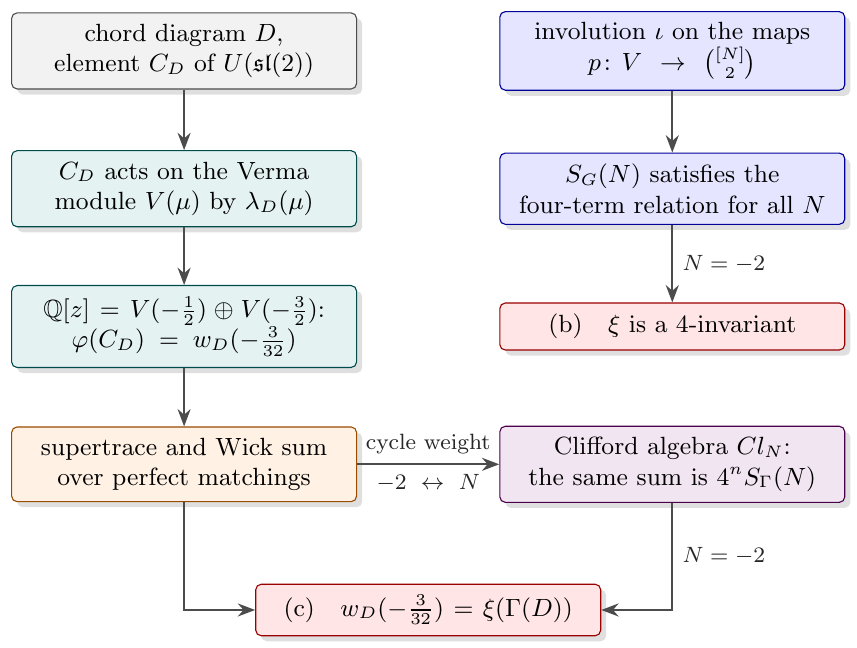
\includegraphics[width=0.9\textwidth]{figures/fig_flow.png}
\caption{The proof of Theorem~\ref{thm:main}. The right column gives part (b), the left column and the bottom row part (c).}\label{fig:flow}
\end{figure}

\section{The weight system and Verma modules}\label{sec:verma}

\subsection{Chord diagrams and the weight system}
A chord diagram with $n$ chords is a fixed-point-free involution $\sigma$ of $[2n]$; its chords are the pairs $\{p,\sigma(p)\}$. It is a chord diagram on an oriented circle cut at a point that is not an endpoint; cutting at another point rotates $[2n]$ cyclically. Chords $\{p<q\}$ and $\{p'<q'\}$ cross if $p<p'<q<q'$ or $p'<p<q'<q$. The intersection graph $\Gamma(D)$ has the chords as vertices and the crossing pairs as edges; it does not depend on the cut.

Let $\g=\slt$ over $\Q$ with basis $E,F,H$, $[H,E]=2E$, $[H,F]=-2F$, $[E,F]=H$, and let
\[
t=\tfrac14\,E\otimes F+\tfrac14\,F\otimes E+\tfrac18\,H\otimes H\in\g\otimes\g
\]
be the Casimir tensor of the Killing form. It is symmetric and $\g$-invariant: $(\operatorname{ad}_x\otimes1+1\otimes\operatorname{ad}_x)t=0$ for $x\in\g$. For a chord diagram $D$ let $t_D\in\g^{\otimes 2n}$ be the tensor with a copy of $t$ in the factors $p,\sigma(p)$ of every chord, and let $C_D\in\Ue$ be the image of $t_D$ under $u_1\otimes\dots\otimes u_{2n}\mapsto u_1\cdots u_{2n}$. For one chord $C_D=C=\frac14(EF+FE+\frac12H^2)$.

For $d\ge1$ let $V_d$ be the irreducible representation of dimension $d$, with basis $e_0,\dots,e_{d-1}$ and
\[
Ee_j=j(d-j)\,e_{j-1},\qquad Fe_j=e_{j+1},\qquad He_j=(d-1-2j)\,e_j,
\]
where $e_{-1}=e_d=0$.
The Casimir element $C$ acts on $V_d$ by $c_d=(d^2-1)/8$. Put $W_d(D)=\tr_{V_d}(C_D)/d$. Rotating the cut permutes the factors of $t_D$ cyclically, so $W_d(D)$ depends only on the diagram on the circle.

By Proposition~\ref{prop:wD} below there is a unique $w_D\in\Q[c]$ with $w_D(c_d)=W_d(D)$ for all $d\ge1$. It is the $\slt$-weight system of \cite{ChV97,FKPU}: by Lemma~\ref{lem:central} $C_D$ lies in the centre of $\Ue$, which is $\Q[C]$ \cite{Hum08}, so $C_D=w(C)$ for a polynomial $w$, and taking traces on $V_d$ gives $w(c_d)=W_d(D)$; the weight system of \cite{FKPU} is defined with the Killing form and takes the value $c$ on one chord.

\begin{lemma}\label{lem:central}
$C_D$ commutes with every $x\in\g$.
\end{lemma}

\begin{proof}
$\operatorname{ad}_x$ is a derivation of $\Ue$, so $[x,C_D]$ is the image of $\sum_{p=1}^{2n}(\operatorname{ad}_x)_p\,t_D$, where $(\operatorname{ad}_x)_p$ acts on the factor $p$. Grouping the two endpoints of every chord writes this sum as a sum over chords of tensors containing $(\operatorname{ad}_x\otimes1+1\otimes\operatorname{ad}_x)t=0$.
\end{proof}

\subsection{Verma modules}
Let $R=\Q[\mu]$ and let $M$ be the free $R$-module with basis $v_0,v_1,\dots$ and
\begin{equation}\label{eq:verma}
Ev_j=j(\mu-j+1)\,v_{j-1},\qquad Fv_j=v_{j+1},\qquad Hv_j=(\mu-2j)\,v_j .
\end{equation}
These operators satisfy the relations of $\g$:
\[
(EF-FE)v_j=\bigl((j+1)(\mu-j)-j(\mu-j+1)\bigr)v_j=(\mu-2j)v_j=Hv_j,
\]
and $(HE-EH)v_j=2Ev_j$, $(HF-FH)v_j=-2Fv_j$, because $H$ has eigenvalue $\mu-2j+2$ on $v_{j-1}$ and $\mu-2j-2$ on $v_{j+1}$. Thus $M$ is a $\Ue$-module on which $\Ue$ acts $R$-linearly. For $\mu_0\in\Q$, specializing $\mu=\mu_0$ gives the Verma module $V(\mu_0)$ of highest weight $\mu_0$.

\begin{proposition}\label{prop:lambda}
There is $\lambda_D\in\Q[\mu]$ with $C_Dm=\lambda_Dm$ for all $m\in M$. Moreover
\begin{enumerate}
\item[(a)] $W_d(D)=\lambda_D(d-1)$ for every $d\ge1$;
\item[(b)] $\lambda_D(\mu)=\lambda_D(-2-\mu)$.
\end{enumerate}
\end{proposition}

\begin{proof}
$H-\mu$ multiplies $v_j$ by $-2j$, so its kernel is $Rv_0$. As $C_D$ commutes with $H$, $C_Dv_0=\lambda_Dv_0$ for some $\lambda_D\in R$, and $C_Dv_j=C_DF^jv_0=F^jC_Dv_0=\lambda_Dv_j$.

(a) In $V(d-1)$, $Ev_d=d(d-1-d+1)v_{d-1}=0$, so $U_d=\operatorname{span}\{v_j:j\ge d\}$ is a submodule. The quotient $V(d-1)/U_d$, with basis the images of $v_0,\dots,v_{d-1}$, is $V_d$ with the formulas above. $C_D$ acts on $V(d-1)$, hence on $V_d$, by $\lambda_D(d-1)$, so $\tr_{V_d}C_D=d\,\lambda_D(d-1)$.

(b) The map $V(-1-d)\to U_d$, $v_j\mapsto v_{d+j}$, is an isomorphism of $\g$-modules: it commutes with $F$; both $Hv_j$ in $V(-1-d)$ and $Hv_{d+j}$ in $V(d-1)$ have eigenvalue $-1-d-2j$; and $Ev_j=j(-d-j)v_{j-1}$ in $V(-1-d)$ while $Ev_{d+j}=(d+j)(-j)v_{d+j-1}$ in $V(d-1)$. Hence $\lambda_D(-1-d)=\lambda_D(d-1)$ for all $d\ge1$, and the polynomial $\lambda_D(\mu)-\lambda_D(-2-\mu)$ has infinitely many roots.
\end{proof}

\begin{proposition}\label{prop:wD}
There is a unique $w_D\in\Q[c]$ with $w_D(c_d)=W_d(D)$ for all $d\ge1$, and $\deg w_D\le n$. It satisfies $\lambda_D(\mu)=w_D\bigl(\mu(\mu+2)/8\bigr)$; in particular
\[
w_D(-\tfrac{3}{32})=\lambda_D(-\tfrac12)=\lambda_D(-\tfrac32).
\]
\end{proposition}

\begin{proof}
By Proposition~\ref{prop:lambda}(b), $\nu\mapsto\lambda_D(\nu-1)$ is even, so $\lambda_D(\nu-1)=g(\nu^2)$ for some $g\in\Q[x]$. Put $w_D(c)=g(8c+1)$. Then $w_D(\mu(\mu+2)/8)=g((\mu+1)^2)=\lambda_D(\mu)$, and $w_D(c_d)=\lambda_D(d-1)=W_d(D)$ by Proposition~\ref{prop:lambda}(a). Uniqueness holds because the $c_d$ are pairwise distinct. Each term of $C_Dv_0$ is obtained by applying $2n$ operators from \eqref{eq:verma}; their coefficients have degree at most one in $\mu$. Thus $\deg\lambda_D\le2n$. Translation by $1$ preserves this degree bound, so $\lambda_D(\nu-1)=g(\nu^2)$ gives $\deg g\le n$, hence $\deg w_D\le n$. In particular $W_d(D)$ for $1\le d\le n+1$ determine $w_D$ by ordinary polynomial interpolation. Finally $\mu(\mu+2)/8=-\frac{3}{32}$ for $\mu=-\frac12$ and for $\mu=-\frac32$.
\end{proof}

\section{The oscillator representation and a supertrace}\label{sec:osc}

Let $A$ be the Weyl algebra over $\Q$ generated by $z$ and $\dd$ with $\dd z-z\dd=1$. It acts faithfully on $\Q[z]$, with $z$ acting by multiplication and $\dd$ by differentiation, and the monomials $z^i\dd^j$ ($i,j\ge0$) form a basis of $A$. In $A$,
\begin{equation}\label{eq:weyl}
z^i\dd^j z=z^{i+1}\dd^j+j\,z^i\dd^{j-1},\qquad \dd\, z^i\dd^j=z^i\dd^{j+1}+i\,z^{i-1}\dd^j .
\end{equation}

\begin{lemma}\label{lem:faithful}
The operators $z^i\dd^j$, $i,j\ge0$, are linearly independent on $\Q[z]$. In particular the action of $A$ on $\Q[z]$ is faithful.
\end{lemma}

\begin{proof}
The relation $\dd z=z\dd+1$ rewrites every word as a linear combination of these operators. Suppose a finite sum $B=\sum_{i,j}a_{ij}z^i\dd^j$ acts by zero. On $z^k$, for all sufficiently large integers $k$, the coefficient of $z^{k+r}$ is
\[
\sum_{i-j=r}a_{ij}\,k(k-1)\cdots(k-j+1).
\]
It vanishes for infinitely many $k$, so it is the zero polynomial in $k$. For each fixed $r$ the falling factorials in this sum have distinct degrees $j$, with leading coefficient $1$; hence every $a_{ij}$ is zero. This also proves that the normal forms are unique, so the action of the abstract Weyl algebra is faithful.
\end{proof}

\begin{lemma}\label{lem:osc}
The assignment $\varphi(E)=-\frac14\dd^2$, $\varphi(F)=z^2$, $\varphi(H)=-\frac12(z\dd+\dd z)$ extends to an algebra homomorphism $\varphi\colon\Ue\to A$. On $\Q[z]$, the maps $v_j\mapsto z^{2j}$ and $v_j\mapsto z^{2j+1}$ are isomorphisms of $\g$-modules $V(-\frac12)\to\Q[z]_{\mathrm{even}}$ and $V(-\frac32)\to\Q[z]_{\mathrm{odd}}$.
\end{lemma}

\begin{proof}
On $\Q[z]$,
\[
Ez^k=-\tfrac14k(k-1)z^{k-2},\qquad Fz^k=z^{k+2},\qquad Hz^k=-(k+\tfrac12)z^k .
\]
Hence $(EF-FE)z^k=-\frac14\bigl((k+2)(k+1)-k(k-1)\bigr)z^k=Hz^k$, and $(HE-EH)z^k=2Ez^k$, $(HF-FH)z^k=-2Fz^k$, because $H$ has eigenvalue $-(k-\frac32)$ on $z^{k-2}$ and $-(k+\frac52)$ on $z^{k+2}$. The relations of $\g$ hold on $\Q[z]$, hence in $A$. For $k=2j$ the formulas read $Ez^{2j}=j(-\frac12-j+1)z^{2j-2}$ and $Hz^{2j}=(-\frac12-2j)z^{2j}$, which is \eqref{eq:verma} at $\mu=-\frac12$; for $k=2j+1$ they read $Ez^{2j+1}=j(-\frac32-j+1)z^{2j-1}$ and $Hz^{2j+1}=(-\frac32-2j)z^{2j+1}$, which is \eqref{eq:verma} at $\mu=-\frac32$.
\end{proof}

\begin{proposition}\label{prop:scalar}
$\varphi(C_D)=w_D(-\frac{3}{32})\cdot1$ in $A$.
\end{proposition}

\begin{proof}
By Proposition~\ref{prop:lambda} and Lemma~\ref{lem:osc}, $\varphi(C_D)$ acts on $\Q[z]_{\mathrm{even}}$ by $\lambda_D(-\frac12)$ and on $\Q[z]_{\mathrm{odd}}$ by $\lambda_D(-\frac32)$. Both equal $w_D(-\frac{3}{32})$ by Proposition~\ref{prop:wD}, and Lemma~\ref{lem:faithful} gives faithfulness.
\end{proof}

Let $\tau\colon A\to\Q$ be the linear map with
\[
\tau(z^i\dd^j)=\delta_{ij}\,(-1)^j\,\frac{j!}{2^j}.
\]
Since $z^j\dd^j$ multiplies $z^k$ by $k(k-1)\cdots(k-j+1)$ and $\sum_kk(k-1)\cdots(k-j+1)x^k=j!\,x^j(1-x)^{-j-1}$, $\tau(a)$ is twice the Abel sum $\lim_{x\to-1^+}\sum_k a_{kk}x^k$ of the supertrace of $a$ on $\Q[z]$, where $az^k=a_{kk}z^k+(\text{other powers})$. Only the following properties are used.

\begin{lemma}\label{lem:tau}
\begin{enumerate}
\item[(a)] $\tau(1)=1$.
\item[(b)] $\tau(xa)=-\tau(ax)$ for $x\in\{z,\dd\}$ and $a\in A$.
\item[(c)] For $u_1,\dots,u_m\in\{z,\dd\}$,
\[
\tau(u_1\cdots u_m)=\sum_{M}\ \prod_{\{a<b\}\in M}\tfrac12\,[u_a,u_b],
\]
the sum over the perfect matchings $M$ of $[m]$; here $[z,\dd]=-1$, $[\dd,z]=1$ and $[z,z]=[\dd,\dd]=0$. For odd $m$ both sides vanish.
\end{enumerate}
\end{lemma}

\begin{proof}
(a) is the case $i=j=0$. For (b) it suffices to take $a=z^i\dd^j$. By \eqref{eq:weyl}, $\tau(z^i\dd^jz)=\tau(z^{i+1}\dd^j)+j\,\tau(z^i\dd^{j-1})$. Both terms vanish unless $j=i+1$, and then the sum is $(-1)^j\frac{j!}{2^j}+j(-1)^{j-1}\frac{(j-1)!}{2^{j-1}}=-(-1)^j\frac{j!}{2^j}=-\tau(z\cdot z^i\dd^j)$. Likewise $\tau(\dd z^i\dd^j)=\tau(z^i\dd^{j+1})+i\,\tau(z^{i-1}\dd^j)$ vanishes unless $i=j+1$, and then it equals $(-1)^{j+1}\frac{(j+1)!}{2^{j+1}}+(j+1)(-1)^j\frac{j!}{2^j}=(-1)^j\frac{(j+1)!}{2^{j+1}}=-\tau(z^i\dd^j\cdot\dd)$.

(c) Induction on $m$. For $m=0$ use (a); for $m=1$, $\tau(z)=\tau(\dd)=0$. For $m\ge2$, as the $[u_1,u_s]$ are scalars,
\[
u_1u_2\cdots u_m=\sum_{s=2}^m[u_1,u_s]\,u_2\cdots\widehat{u_s}\cdots u_m+u_2\cdots u_mu_1 .
\]
Applying $\tau$ and (b) to the last term gives
\[
\tau(u_1\cdots u_m)=\tfrac12\sum_{s=2}^m[u_1,u_s]\,\tau(u_2\cdots\widehat{u_s}\cdots u_m),
\]
which is the expansion of the right side of (c) according to the partner $s$ of $1$.
\end{proof}

\begin{corollary}\label{cor:tau}
$w_D(-\frac{3}{32})=\tau(\varphi(C_D))$.
\end{corollary}

\section{Expansion over matchings}\label{sec:matching}

\subsection{Matchings}
Let $X$ be a finite totally ordered set and $P,M$ perfect matchings of $X$. Two edges $\{a<b\}$ and $\{a'<b'\}$ cross if $a<a'<b<b'$ or $a'<a<b'<b$, and $\cro(P)$ is the number of crossing pairs of edges of $P$. The multigraph $P\cup M$ is a disjoint union of cycles alternating between edges of $P$ and of $M$ (a common edge gives a cycle of length $2$); $\cyc(P,M)$ is their number. Orient every cycle; an edge oriented from a larger to a smaller element is a descent, and $\des(P,M)$ is the number of descents. Reversing a cycle of length $2r$ turns $\delta$ descents into $2r-\delta$, so the parity of $\des(P,M)$ does not depend on the orientations. Put
\[
L_P(N)=\sum_M(-1)^{\cro(M)}N^{\cyc(P,M)}\in\Z[N],
\]
the sum over all perfect matchings $M$ of $X$.

\begin{lemma}\label{lem:sign}
$\cro(P)+\cro(M)+\cyc(P,M)+\des(P,M)$ is even.
\end{lemma}

\begin{proof}
Let $Q(P,M)$ be the sum. Let $x<y$ be consecutive in $X$, and exchange their positions in the order, keeping $P$ and $M$. If $\{x,y\}\notin P$, let $e\ni x$ and $f\ni y$ be the edges of $P$; the exchange moves $y$ to the other side of the endpoint $x$ of $e$ and keeps the side of the other endpoint of $f$, so it changes whether $e$ and $f$ cross, and no other pair. Thus $\cro(P)$ changes by $1-[\{x,y\}\in P]$ modulo $2$, and likewise $\cro(M)$. $\cyc(P,M)$ does not change. A descent status changes only on edges joining $x$ and $y$, so $\des(P,M)$ changes by $[\{x,y\}\in P]+[\{x,y\}\in M]$. The total change is $2$. Any two total orders of $X$ are related by exchanges of consecutive elements, so $Q$ modulo $2$ is the same for all orders. Choose an order in which every cycle $x_1x_2\cdots x_{2r}$ (with $x_1x_2\in P$) occupies consecutive positions in this order. Then $P$ and $M$ have no crossings, and each cycle, oriented as listed, has exactly one descent, from $x_{2r}$ to $x_1$. Hence $Q\equiv2\cyc(P,M)\equiv0$.
\end{proof}

\subsection{The bosonic expansion}
For a perfect matching $P$ of $X$ with $k$ edges let
\[
X_P=\sum_{o}\operatorname{sgn}(o)\prod_{x\in X}^{\longrightarrow}u^o_x\in A,
\]
the sum over the $2^k$ orientations $o$ of the edges of $P$, where $u^o_x=z$ if $x$ is the tail of its edge and $u^o_x=\dd$ if it is the head, the product is taken in the order of $X$, and $\operatorname{sgn}(o)=(-1)^{\text{number of descents of }o}$.

\begin{proposition}\label{prop:boson}
$\tau(X_P)=2^{-k}(-1)^{\cro(P)}L_P(-2)$.
\end{proposition}

\begin{proof}
By Lemma~\ref{lem:tau}(c),
\[
\tau(X_P)=\sum_o\sum_M\operatorname{sgn}(o)\prod_{\{a<b\}\in M}\tfrac12[u^o_a,u^o_b].
\]
A term vanishes unless every edge of $M$ joins a head and a tail of $o$. Orient such an edge from the head to the tail; then $\frac12[u^o_a,u^o_b]$ is $\frac12$ if it is oriented from $a$ to $b$ ($u^o_a=\dd$, $u^o_b=z$) and $-\frac12$ if it is a descent. As $\operatorname{sgn}(o)$ is $-1$ to the number of descents among the edges of $P$, the term equals $2^{-k}(-1)^{\des(P,M)}$. Every element of $X$ is then entered by exactly one oriented edge and left by exactly one, so the cycles of $P\cup M$ are directed cycles. Conversely, each of the $2^{\cyc(P,M)}$ orientations of the cycles of $P\cup M$ as directed cycles restricts on $P$ to an orientation $o$ for which every edge of $M$ joins a head to a tail. Hence
\begin{align*}
\tau(X_P)&=2^{-k}\sum_M2^{\cyc(P,M)}(-1)^{\des(P,M)}\\
&=2^{-k}(-1)^{\cro(P)}\sum_M(-1)^{\cro(M)}(-2)^{\cyc(P,M)}
\end{align*}
by Lemma~\ref{lem:sign}.
\end{proof}

\subsection{Legs}
Let $D$ be a chord diagram with $n$ chords. Every point $p\in[2n]$ carries two legs $(p,1)<(p,2)$, and the set $X_D$ of the $4n$ legs is ordered lexicographically. For a chord $c=\{p<q\}$ and $\beta\in\{0,1\}$ let $P_c^\beta$ be the pair of edges
\[
P_c^0=\{(p,1)(q,1),\ (p,2)(q,2)\},\qquad P_c^1=\{(p,1)(q,2),\ (p,2)(q,1)\},
\]
and for $\beta\colon\{\text{chords}\}\to\{0,1\}$ let $P_\beta=\bigcup_cP_c^{\beta(c)}$, a perfect matching of $X_D$. Let $\pi=z\otimes\dd-\dd\otimes z\in A\otimes A$. Writing $\pi=\sum_r\varepsilon_r\,x_r\otimes y_r$, put $\pi_{13}\pi_{24}=\sum_{r,s}\varepsilon_r\varepsilon_s\,x_rx_s\otimes y_ry_s$ and $\pi_{14}\pi_{23}=\sum_{r,s}\varepsilon_r\varepsilon_s\,x_rx_s\otimes y_sy_r$.

\begin{lemma}\label{lem:pi}
$(\varphi\otimes\varphi)(t)=-\frac{1}{32}\bigl(\pi_{13}\pi_{24}+\pi_{14}\pi_{23}\bigr)$.
\end{lemma}

\begin{proof}
Both sides equal $-\frac1{32}\bigl(2z^2\otimes\dd^2+2\dd^2\otimes z^2-(z\dd+\dd z)\otimes(z\dd+\dd z)\bigr)$. On the left, $\frac14\varphi(E)\otimes\varphi(F)+\frac14\varphi(F)\otimes\varphi(E)=-\frac1{16}(\dd^2\otimes z^2+z^2\otimes\dd^2)$ and $\frac18\varphi(H)\otimes\varphi(H)=\frac1{32}(z\dd+\dd z)^{\otimes2}$. On the right, the terms with $r=s$ give $2z^2\otimes\dd^2+2\dd^2\otimes z^2$ and the terms with $r\ne s$ give $-z\dd\otimes(\dd z+z\dd)-\dd z\otimes(z\dd+\dd z)$.
\end{proof}

\begin{corollary}\label{cor:legs}
$\varphi(C_D)=\bigl(-\frac{1}{32}\bigr)^n\sum_\beta X_{P_\beta}$, the sum over all $\beta\colon\{\text{chords}\}\to\{0,1\}$.
\end{corollary}

\begin{proof}
$\varphi(C_D)$ is the product, in the order of the points, of the factors of $(\varphi\otimes\varphi)(t)^{\otimes n}$ placed at the endpoints of the chords. Put the two letters of each factor $x_rx_s$ or $y_ry_s$ on the two legs of its point, in this order. By Lemma~\ref{lem:pi}, a chord contributes $-\frac1{32}$ times the sum of $\pi$ placed on the two edges of $P_c^0$ and $\pi$ placed on the two edges of $P_c^1$. A copy of $\pi$ on an edge $\{a<b\}$ contributes $z$ at $a$ and $\dd$ at $b$ with sign $+1$, or $\dd$ at $a$ and $z$ at $b$ with sign $-1$; these are the two orientations of the edge with their signs in $X_{P_\beta}$.
\end{proof}

\section{Clifford algebras}\label{sec:clifford}

For $N\ge1$ let $Cl_N$ be the $\Q$-algebra generated by $e_1,\dots,e_N$ with $e_ie_j+e_je_i=2\delta_{ij}$. For $I=\{i_1<\dots<i_r\}\subseteq[N]$ put $e_I=e_{i_1}\cdots e_{i_r}$; these form a basis, and $e_Ie_J=\pm e_{I\triangle J}$. Let $\tr\colon Cl_N\to\Q$ be linear with $\tr(e_I)=\delta_{I\emptyset}$. Then $\tr(ab)=\tr(ba)$: for basis elements both sides vanish unless $I=J$.

\begin{lemma}\label{lem:cliffwick}
For $i_1,\dots,i_m\in[N]$,
\[
\tr(e_{i_1}\cdots e_{i_m})=\sum_M(-1)^{\cro(M)}\prod_{\{a,b\}\in M}\delta_{i_ai_b},
\]
the sum over the perfect matchings $M$ of $[m]$.
\end{lemma}

\begin{proof}
For odd $m$ the product is $\pm e_I$ with $|I|$ odd, so both sides vanish. For even $m\ge2$, moving $e_{i_1}$ to the right end gives
\[
e_{i_1}e_{i_2}\cdots e_{i_m}=\sum_{s=2}^m(-1)^{s}\,2\delta_{i_1i_s}\,e_{i_2}\cdots\widehat{e_{i_s}}\cdots e_{i_m}-e_{i_2}\cdots e_{i_m}e_{i_1}.
\]
Taking traces and using $\tr(e_{i_2}\cdots e_{i_m}e_{i_1})=\tr(e_{i_1}\cdots e_{i_m})$,
\[
\tr(e_{i_1}\cdots e_{i_m})=\sum_{s=2}^m(-1)^s\delta_{i_1i_s}\tr(e_{i_2}\cdots\widehat{e_{i_s}}\cdots e_{i_m}).
\]
The edge $\{1,s\}$ crosses exactly the edges with one endpoint in $\{2,\dots,s-1\}$; the elements of this set matched among themselves come in pairs, so the number of such edges is congruent to $s-2$. By induction both sides satisfy the same recursion.
\end{proof}

\begin{corollary}\label{cor:colour}
For a perfect matching $P$ of a totally ordered set $X=\{x_1<\dots<x_{2k}\}$ and $N\ge1$,
\[
\sum_\kappa\tr(e_{\kappa(x_1)}\cdots e_{\kappa(x_{2k})})=L_P(N),
\]
the sum over the maps $\kappa\colon X\to[N]$ that are constant on every edge of $P$.
\end{corollary}

\begin{proof}
By Lemma~\ref{lem:cliffwick} the left side is $\sum_M(-1)^{\cro(M)}$ times the number of maps $X\to[N]$ constant on the edges of $P$ and of $M$, which is $N^{\cyc(P,M)}$.
\end{proof}

For $I=\{i<j\}\in\binomset{[N]}{2}$ write $b_I=e_ie_j$. Then
\begin{equation}\label{eq:bivector}
b_Ib_J=(-1)^{|I\cap J|}\,b_Jb_I,\qquad b_I^2=-1 .
\end{equation}

\begin{proposition}\label{prop:clifford}
Let $D$ be a chord diagram with $n$ chords and $\Gamma=\Gamma(D)$. Then
\[
\sum_\beta(-1)^{\cro(P_\beta)}L_{P_\beta}(N)=4^n\,S_\Gamma(N)
\]
as polynomials in $N$.
\end{proposition}

\begin{proof}
Both sides are polynomials (Theorem~\ref{thm:main}(a) is proved in Section~\ref{sec:proof} independently), so it suffices to take $N\ge1$.

The two edges of $P_c^\beta$ cross if and only if $\beta=0$. If chords $c$ and $c'$ cross, every edge of $P_c^\beta$ crosses every edge of $P_{c'}^{\beta'}$; otherwise none does. Hence
\[
(-1)^{\cro(P_\beta)}=(-1)^n\prod_c(-1)^{\beta(c)}.
\]

A map $\kappa$ constant on the edges of $P_\beta$ is given by a pair $(i_c,j_c)\in[N]^2$ for every chord $c=\{p<q\}$: $i_c$ on the edge through $(p,1)$ and $j_c$ on the edge through $(p,2)$. The legs at $p$ then read $e_{i_c}e_{j_c}$, and the legs at $q$ read $e_{i_c}e_{j_c}$ if $\beta(c)=0$ and $e_{j_c}e_{i_c}$ if $\beta(c)=1$. By Corollary~\ref{cor:colour}, summing over $\beta(c)$ with the sign $(-1)^{\beta(c)}$ replaces the factor at $q$ by $e_{i_c}e_{j_c}-e_{j_c}e_{i_c}$, which is $0$ if $i_c=j_c$ and $2e_{i_c}e_{j_c}$ otherwise. Exchanging $i_c$ and $j_c$ changes the sign of both factors of $c$, so every $2$-element set $s(c)=\{i_c,j_c\}$ arises twice with the same value. Therefore
\[
\sum_\beta(-1)^{\cro(P_\beta)}L_{P_\beta}(N)=(-1)^n4^n\sum_{s}\tr(B_s),\qquad B_s=\prod_{p=1}^{2n}b_{s(c_p)},
\]
the sum over $s\colon\{\text{chords}\}\to\binomset{[N]}{2}$, where $c_p$ is the chord through $p$.

We show $\tr(B_s)=(-1)^n\prod_{cc'\in E(\Gamma)}(-1)^{|s(c)\cap s(c')|}$ by induction on $n$. Let $c=\{p<q\}$. Move the factor at $p$ to the right until it is next to the factor at $q$. By \eqref{eq:bivector} it passes the factors at the points strictly between $p$ and $q$; a chord with both endpoints there contributes the square of a sign, and the chords with one endpoint there are the neighbours of $c$ in $\Gamma$. Then $b_{s(c)}^2=-1$, and the remaining word is $B_{s'}$ for the diagram $D\setminus c$, whose intersection graph is $\Gamma-c$, with $s'=s|_{\Gamma-c}$. Summing over $s$ gives $\sum_s\tr(B_s)=(-1)^nS_\Gamma(N)$.
\end{proof}

\section{Proof of Theorem~\ref{thm:main}}\label{sec:proof}

\begin{proof}[Proof of (a)]
Group the maps $p\colon V\to\binomset{[N]}{2}$ by $U=\bigcup_xp(x)$. Relabelling $U$ in increasing order by $[|U|]$ preserves all intersection sizes, so the maps with $|U|=k$ contribute $\binom Nk T_k(G)$; and $T_k(G)=0$ for $k>2n$.
\end{proof}

\begin{proof}[Proof of (c)]
By Corollaries~\ref{cor:tau} and~\ref{cor:legs}, Proposition~\ref{prop:boson} with $k=2n$, and Proposition~\ref{prop:clifford},
\begin{align*}
w_D(-\tfrac{3}{32})&=\Bigl(-\frac{1}{32}\Bigr)^n\sum_\beta\tau(X_{P_\beta})=\Bigl(-\frac{1}{32}\Bigr)^n4^{-n}\sum_\beta(-1)^{\cro(P_\beta)}L_{P_\beta}(-2)\\
&=\frac{S_\Gamma(-2)}{(-32)^n}=\xi(\Gamma).\qedhere
\end{align*}
\end{proof}

For a graph $G$ and distinct vertices $a,b$ let $G'_{ab}$ be $G$ with the adjacency of $a$ and $b$ reversed, and $\widetilde G_{ab}$ be $G$ with the adjacency of $a$ and $y$ reversed for every neighbour $y\ne a$ of $b$. The four-term relation for a function $f$ on graphs is
\[
f(G)-f(G'_{ab})=f(\widetilde G_{ab})-f(\widetilde G'_{ab}),\qquad \widetilde G'_{ab}=(\widetilde G_{ab})'_{ab},
\]
as in Figure~\ref{fig:fourterm}.

\begin{figure}[ht]
\centering
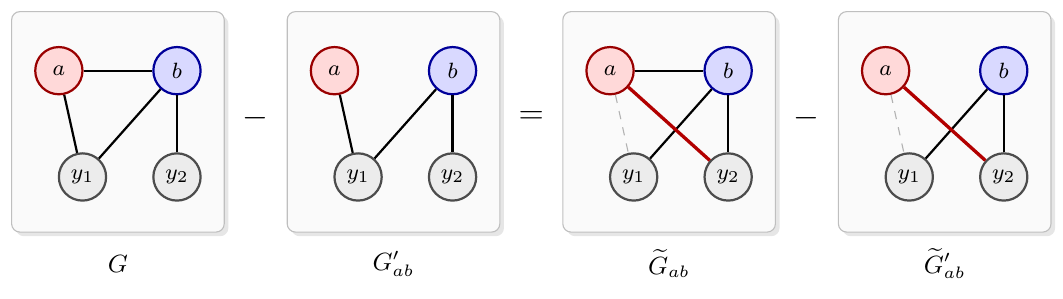
\includegraphics[width=\textwidth]{figures/fig_fourterm.png}
\caption{The four graphs of a four-term relation. Here $b$ has the neighbours $a,y_1,y_2$; passing from $G$ to $\widetilde G_{ab}$ removes the edge $ay_1$ (dashed) and adds the edge $ay_2$.}\label{fig:fourterm}
\end{figure}

\begin{proposition}\label{prop:fourT}
For every $N\in\N$, $G\mapsto S_G(N)$ satisfies the four-term relation.
\end{proposition}

\begin{proof}
For $p\colon V\to\binomset{[N]}{2}$ write
\[
\epsilon(G,p)=\prod_{xy\in E(G)}(-1)^{|p(x)\cap p(y)|}.
\]
Since $\epsilon(G'_{ab},p)=\epsilon(G,p)(-1)^{|p(a)\cap p(b)|}$ and $|p(a)\cap p(b)|\in\{0,1,2\}$,
\[
S_G(N)-S_{G'_{ab}}(N)=2\sum_{p\in\Pi}\epsilon(G,p),\qquad \Pi=\{p:|p(a)\cap p(b)|=1\}.
\]
The construction $\widetilde G_{ab}$ does not change the adjacency of $a$ and $b$, so the same holds for $\widetilde G_{ab}$. On $\Pi$ define $\iota(p)$ by $\iota(p)(b)=p(a)\triangle p(b)$ and $\iota(p)(x)=p(x)$ for $x\ne b$. As $|p(a)\cap p(b)|=1$, $\iota(p)(b)$ is a $2$-element set meeting $p(a)$ in one element, and $\iota$ is an involution of $\Pi$. Let $Y$ be the set of neighbours $y\ne a$ of $b$ in $G$, which is also the set of such neighbours in $\widetilde G_{ab}$. For $y\in Y$, $|(p(a)\triangle p(b))\cap p(y)|\equiv|p(a)\cap p(y)|+|p(b)\cap p(y)|$, and the edge $ab$, if present, keeps its sign because $|p(a)\cap\iota(p)(b)|=1$. Hence
\begin{gather*}
\epsilon(G,\iota(p))=\epsilon(G,p)\prod_{y\in Y}(-1)^{|p(a)\cap p(y)|},\\
\epsilon(\widetilde G_{ab},q)=\epsilon(G,q)\prod_{y\in Y}(-1)^{|q(a)\cap q(y)|},
\end{gather*}
the second for every $q$ since $\widetilde G_{ab}$ differs from $G$ exactly in the pairs $ay$, $y\in Y$. With $q=\iota(p)$, which agrees with $p$ at $a$ and on $Y$, this gives $\epsilon(\widetilde G_{ab},\iota(p))=\epsilon(G,p)$. Therefore $\sum_{p\in\Pi}\epsilon(\widetilde G_{ab},p)=\sum_{p\in\Pi}\epsilon(G,p)$, and the two differences agree.
\end{proof}

\begin{proof}[Proof of (b)]
$\xi$ depends only on the isomorphism class of $G$. The four graphs of a four-term relation have the same vertex set, so by Proposition~\ref{prop:fourT} and (a) the four-term relation holds for the polynomials $S_G$, hence at $N=-2$, and after division by $(-32)^n$ for $\xi$.
\end{proof}

\begin{remark}
Proposition~\ref{prop:fourT} applied to the sets $\Pi$ restricted to the maps with $\bigcup_xp(x)=[k]$, which $\iota$ preserves, shows that every $T_k$ satisfies the four-term relation. By the proof of Proposition~\ref{prop:clifford}, for $N\ge1$ the $4$-invariant $S_\Gamma(N)$ is $(-4)^{-n}$ times the Clifford trace of the element obtained by placing the tensor $\sum_{i\ne j}e_ie_j\otimes 2e_ie_j$ on the chords as in the definition of $C_D$, and Theorem~\ref{thm:main}(c) identifies $w_D(-\frac{3}{32})$ with $(-32)^{-n}$ times its value at $N=-2$.
\end{remark}

\section{Formal verification}\label{sec:lean}

Parts (b) and (c) of Theorem~\ref{thm:main} are formalized in Lean~4 \cite{MU21} with Mathlib \cite{Mathlib20}, version~4.34.1, and the formal proof is checked by the Lean kernel. The formal statement has two parts. The first says that $\xi$ is invariant under isomorphisms of graphs and satisfies the four-term relation for every graph and every pair of distinct vertices $a,b$. The second says that for every chord diagram $D$ there is a polynomial $P\in\Q[c]$ with $P(c_d)=W_d(D)$ for all $d\ge1$, and that every such polynomial, that is $w_D$, takes the value $\xi(\Gamma(D))$ at $c=-\frac{3}{32}$. A chord diagram is a fixed-point-free involution of $\{0,\dots,2n-1\}$, the trace $W_d(D)$ is computed from the matrices of $E,F,H$ on $V_d$ in the basis of Section~\ref{sec:verma}, and $\Gamma(D)$, $G'_{ab}$, $\widetilde G_{ab}$, $T_k$ and $\xi$ are as in Sections~\ref{sec:intro} and~\ref{sec:proof}. The proof depends only on the axioms of Lean's logic, namely propositional extensionality, choice and the soundness of quotients; it has no unproved step and adds no axiom.

The formal proof follows Sections~\ref{sec:verma}--\ref{sec:proof} with three changes of route. Proposition~\ref{prop:lambda}(b) is derived from an identity between the coefficients of words acting on the Verma modules of highest weights $\mu$ and $-2-\mu$, which is the isomorphism $V(-1-d)\cong U_d$ in coordinates. The identity $W_d(D)=\lambda_D(d-1)$ is proved by expanding matrix entries of words over paths. The sums over matchings are encoded by a loop polynomial of a word in which every label occurs twice, defined by contracting the first label; the bosonic expansion (Proposition~\ref{prop:boson}) and the Clifford colour sum (Corollary~\ref{cor:colour}, with the Clifford trace realized as $(-1)$ to the number of inversions of a word in which every letter occurs an even number of times) are shown to satisfy the same recursion, which replaces Lemma~\ref{lem:sign}.

Independent computations confirm the theorem on small cases. In exact rational arithmetic, $w_D(-\frac{3}{32})$, obtained by interpolating $W_d(D)$ for $d\le n+1$, agrees with $\xi(\Gamma(D))$ on all chord diagrams with at most $5$ chords and on random larger ones, the four-term relation holds on all graphs with at most $4$ vertices, and each identity of Sections~\ref{sec:osc}--\ref{sec:clifford} holds on small cases. Modulo the prime $2^{61}-1$, the two sides agree on all $11465$ chord diagrams with at most $6$ chords and on $400$ random diagrams with $7$ and $8$ chords, the four-term relation holds on all graphs with at most $5$ vertices, and $\xi$ reproduces the values of the extension tabulated in \cite{FKPU} on $63$ graphs with $9$ and $10$ vertices.

\subsection*{Scope and completeness of the construction}
The formula for $\xi$ is a finite formula for every finite graph, with no bound on its number of vertices: $T_k(G)=0$ for $k>2|V(G)|$. The involution in Proposition~\ref{prop:fourT} is defined on every assignment with $|p(a)\cap p(b)|=1$ and preserves the set of colours used. Thus its proof does not require a finite table of graphs. Similarly, the identities in Sections~\ref{sec:verma}--\ref{sec:clifford} hold for every chord diagram, rather than just those in the numerical checks. Polynomial evaluation at $N=-2$ in the proof of (c) means substitution into a finite polynomial; no limit, analytic continuation or infinite-dimensional trace convergence is assumed. The finite-dimensional normalized traces $W_d(D)$ are the starting definition, and the Verma-module argument proves their unique polynomial interpolation before its oscillator value is evaluated. Consequently the construction proves the whole extension conjecture at $c=-3/32$. It does not assert that the unspecialized $\mathfrak{sl}(2)$ weight system extends to all graphs; that assertion is false by~\cite{FKPU}.

The source definitions of the formal theorem use actual matrices for $E,F,H$, their normalized Casimir trace $W$, alternating endpoints for the intersection graph, and the signed surjective counts $T_k$ for $\xi$. In particular $W$ is not defined by the proposed graph formula. The axiom reports therefore accompany a check of the definitions as well as a check of proof terms. The hand proof of part (a) is the direct grouping by the used colour set; the formal development also contains that counting identity as \texttt{sum\_card\_two} and the binomial polynomial as \texttt{Sp}. The release records distinguish this coverage from the two conjuncts of \texttt{main\_theorem}. The elementary normal-form argument of Lemma~\ref{lem:faithful} is supplied in the written proof; it is not a claim of a new Lean formalization of the abstract Weyl algebra.

\section*{Data and code availability}
\begingroup\raggedright
The \LaTeX{} source of the paper, the Lean~4 formalization of Theorem~\ref{thm:main}(b) and~(c) and the programs of Section~\ref{sec:lean} are in release~v2.2.0 of the repository \url{https://github.com/creelie/automatic-memory} \cite{archive}. The original proof, text and verification code were developed by Deep Bhattacharjee with AI assistance (Claude, Anthropic), as recorded with the earlier preprint. The present revision adds an elementary normal-form proof, clarifies the universal scope and records a definition audit and exact verification evidence. Its release includes the proof source, pinned toolchain and verification receipts.\par
\endgroup

\section*{Declaration of generative AI and AI-assisted technologies}
Claude (Anthropic) assisted the original mathematical exploration, proof drafting, text, figures, Lean development and checking programs. OpenAI Codex assisted the present proof review, the added normal-form argument, literature checks, verification records and preparation of the manuscript and submission files. These uses include research assistance as well as manuscript preparation. Human authors are responsible for the mathematics, references, final text and submission decisions; AI tools are not authors. The accompanying provenance record identifies the checks and their scope.

\section*{Ethical declarations}
Funding: none. Competing interests: none.

\begin{thebibliography}{10}
\raggedright
\expandafter\ifx\csname url\endcsname\relax
  \def\url#1{\texttt{#1}}\fi
\expandafter\ifx\csname urlprefix\endcsname\relax\def\urlprefix{URL }\fi
\expandafter\ifx\csname href\endcsname\relax
  \def\href#1#2{#2} \def\path#1{#1}\fi

\bibitem{Kon93}
M.~Kontsevich, Vassiliev's knot invariants, in: I. M. Gel'fand Seminar, Vol.
  16, Part 2 of Adv. Soviet Math., Amer. Math. Soc., Providence, RI, 1993, pp.
  137--150.
\newblock \href {https://doi.org/10.1090/advsov/016.2/04}
  {\path{doi:10.1090/advsov/016.2/04}}.

\bibitem{BN95}
D.~Bar-Natan, On the {V}assiliev knot invariants, Topology 34~(2) (1995)
  423--472.
\newblock \href {https://doi.org/10.1016/0040-9383(95)93237-2}
  {\path{doi:10.1016/0040-9383(95)93237-2}}.

\bibitem{CDM12}
S.~Chmutov, S.~Duzhin, J.~Mostovoy, Introduction to {V}assiliev Knot
  Invariants, Cambridge University Press, Cambridge, 2012.
\newblock \href {https://doi.org/10.1017/CBO9781139107846}
  {\path{doi:10.1017/CBO9781139107846}}.

\bibitem{ChL07}
S.~Chmutov, S.~Lando, Mutant knots and intersection graphs, Algebr. Geom.
  Topol. 7~(3) (2007) 1579--1598.
\newblock \href {https://doi.org/10.2140/agt.2007.7.1579}
  {\path{doi:10.2140/agt.2007.7.1579}}.

\bibitem{Lan00}
S.~K. Lando, On a {H}opf algebra in graph theory, J. Combin. Theory Ser. B
  80~(1) (2000) 104--121.
\newblock \href {https://doi.org/10.1006/jctb.2000.1973}
  {\path{doi:10.1006/jctb.2000.1973}}.

\bibitem{KL22}
M.~E. Kazarian, S.~K. Lando, Weight systems and invariants of graphs and
  embedded graphs, Russian Math. Surveys 77~(5) (2022) 893--942.
\newblock \href {https://doi.org/10.4213/rm10054e}
  {\path{doi:10.4213/rm10054e}}.

\bibitem{Kra21}
E.~Krasilnikov, An extension of the {$\mathfrak{sl}_2$} weight system to graphs
  with $n \le 8$ vertices, Arnold Math. J. 7 (2021) 609--618.
\newblock \href {https://doi.org/10.1007/s40598-021-00187-7}
  {\path{doi:10.1007/s40598-021-00187-7}}.

\bibitem{FKPU}
D.~Fomichev, M.~Karev, F.~Pavutnitskiy, S.~Usanov, {$\mathfrak{sl}(2)$}-weight
  system does not extend to a graph 4-invariant, arXiv:2607.24217, data:
  \url{https://github.com/fomichev-d/sl2_at_-3_32} (2026).

\bibitem{FK25}
D.~Fomichev, M.~Karev, The {$\mathfrak{sl}(2)$}-weight system at $c = 3/8$ for
  graphs, European J. Combin. 127 (2025) 104160.
\newblock \href {https://doi.org/10.1016/j.ejc.2025.104160}
  {\path{doi:10.1016/j.ejc.2025.104160}}.

\bibitem{YDJ26}
Q.~Yan, Q.~Deng, X.~Jin, Proof of a conjecture of {F}omichev and {K}arev,
  European J. Combin. 135 (2026) 104365.
\newblock \href {https://doi.org/10.1016/j.ejc.2026.104365}
  {\path{doi:10.1016/j.ejc.2026.104365}}.

\bibitem{ChV97}
S.~V. Chmutov, A.~N. Varchenko, Remarks on the {V}assiliev knot invariants
  coming from {$\mathfrak{sl}_2$}, Topology 36~(1) (1997) 153--178.
\newblock \href {https://doi.org/10.1016/0040-9383(95)00071-2}
  {\path{doi:10.1016/0040-9383(95)00071-2}}.

\bibitem{Hum08}
J.~E. Humphreys, Representations of Semisimple {L}ie Algebras in the {BGG}
  Category {$\mathcal{O}$}, Vol.~94 of Grad. Stud. Math., Amer. Math. Soc.,
  Providence, RI, 2008.
\newblock \href {https://doi.org/10.1090/gsm/094} {\path{doi:10.1090/gsm/094}}.

\bibitem{MU21}
L.~de~Moura, S.~Ullrich, The {L}ean 4 theorem prover and programming language,
  in: Automated Deduction -- CADE 28, Vol. 12699 of Lecture Notes in Comput.
  Sci., Springer, Cham, 2021, pp. 625--635.
\newblock \href {https://doi.org/10.1007/978-3-030-79876-5_37}
  {\path{doi:10.1007/978-3-030-79876-5_37}}.

\bibitem{Mathlib20}
{The mathlib Community}, The {L}ean mathematical library, in: Proceedings of
  the 9th ACM SIGPLAN International Conference on Certified Programs and
  Proofs, ACM, New York, 2020, pp. 367--381.
\newblock \href {https://doi.org/10.1145/3372885.3373824}
  {\path{doi:10.1145/3372885.3373824}}.


\bibitem{archive}
D.~Bhattacharjee, U.~Bhattacharya, The $\mathfrak{sl}(2)$ weight system at $c=-3/32$ extends to a graph 4-invariant: Lean 4 formalization and verification code, release v2.2.0 (2026).
\newblock \url{\releaseURL}.

\end{thebibliography}

\end{document}
